\newpage \subsection*{Ασκηση 3}

Να εξομοιωθεί η λειτουργία ενός υποθετικού \en{I.C.} που περιλαμβανει 5 πύλες όπως φαίνεται στο σχήμα. Τα \en{bits} εισόδου
πρέπει να αντιστοιχούν ακριβώς όπως φαίνονται στο σχήμα με τα \en{dip switches} της πόρτας εισόδου \en{2000 Hex}, και οι 
έξοδοι με τα \en{LEDs} που πρέπει να είναι τα τέσσερα \en{LSB} της πόρτας εξόδου \en{3000 Hex}. Οι πύλες, όπως φαίνονται
στο σχήμα, είναι 2 \en{AND}, 2 \en{OR} και 1 \en{XOR}. Η αντιστοιχία των \en{led} με τις λογικές στάθμες έχει ως εξής:
αναμμένο \en{led} $\Rightarrow$ ''1'' και σβηστό \en{led} $\Rightarrow$ ''0''. Οι αδιάφορες θέσεις της εξόδου να έχουν μόνιμα σβηστά \en{led}.

\begin{center}
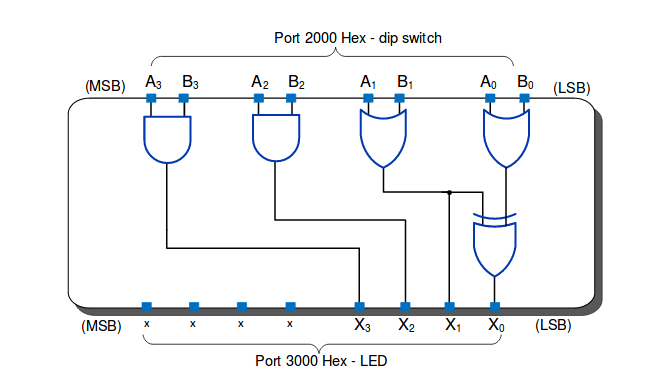
\includegraphics[width=.5\textwidth]{./ex3/Selection_007.png}
\end{center}

\subsubsection*{Λύση}

\selectlanguage{english}
\inputminted{text}{./ex3/ex3.8085}
\selectlanguage{greek}



